\documentclass[12pt,a4paper]{article}
\usepackage{amsfonts,amsmath,amsthm, graphicx, hyperref}
\usepackage[utf8x]{inputenc}
\usepackage[table,xcdraw]{xcolor}
\usepackage{listings}
\usepackage{xcolor}
\usepackage{pgf-pie}
%Path relative to the .tex file containing the \includegraphics command
\graphicspath{ {images/} }
\usepackage[normalem]{ulem}
\useunder{\uline}{\ul}{}
\hypersetup{
	colorlinks=true,
	linkcolor=black,
	filecolor=black,      
	urlcolor=blue,
}
\definecolor{codegreen}{rgb}{0,0.6,0}
\definecolor{codegray}{rgb}{0.5,0.5,0.5}
\definecolor{codepurple}{rgb}{0.58,0,0.82}
\definecolor{backcolour}{rgb}{0.95,0.95,0.92}

\lstdefinestyle{mystyle}{
	backgroundcolor=\color{backcolour},   
	commentstyle=\color{codegreen},
	keywordstyle=\color{magenta},
	numberstyle=\tiny\color{codegray},
	stringstyle=\color{codepurple},
	basicstyle=\ttfamily\footnotesize,
	breakatwhitespace=false,         
	breaklines=true,                 
	captionpos=b,                    
	keepspaces=true,                 
	numbers=left,                    
	numbersep=5pt,                  
	showspaces=false,                
	showstringspaces=false,
	showtabs=false,                  
	tabsize=2
}

\lstset{style=mystyle}
\title{\bf Robotic mobile manipulator}

\renewcommand*\contentsname{Cuprins}

\author{Cristian Bălan}
\date{\today}

\begin{document}
	\maketitle
	
	\pagebreak
	
	\tableofcontents
	
	\pagebreak
	
	\section{Introducere}
	
	\par Proiectul a fost gândit sa ajute navigarea și parcurgerea zonelor periculoase cu un robot de la o distanta mare de acea zona. VR-ul și mediul virtual este folosit ca sa ajute percepția robotului pentru utilizator și de a controla mai ușor robotul.
	
	\par Aplicația trebuie să iți permită să folosești un "VR headset" cu controale (în prezent fiind testat numai pe ce am folosit la dezvoltare, acesta fiind Oculus Rift). 
	
	\par O să am robotul fizic în viața reală si o clonă de a sa în mediul virtual. Trebuie să se miște la fel ambii roboți ca să trebuiască să te folosești doar de mediul virtual ca să navighezi robotul din realitate.
	
	\par Robotul o să fie controlat prin Bluetooth și o să fie configurat folosind Arduino IDE. Placa configurabila de pe robot este un Mega PI și merge să fie configurat cu Arduino IDE. Există si librarii librării pentru folosirea motoarelor si a senzorilor pe Arduino create special pentru modelul de robot folosit.
	
	\par În prezent robotul are roți cu care să navigheze, un motor pentru a mișca mana mai sus sau mai jos si o gheara care se poate închide/deschide, iar pentru senzori are un giroscop și un senzor pentru detectarea distanței dintre el și obiectul din fata (pana la maxim 400 de centimetri). Cu giroscopul din robot se pot trimite informații la mediul virtual despre cum e rotit in robotul în viața reala iar cu celălalt senzor, ultrasunete, se poate construi lumea virtuală după ce observă robotul.
	
	\par În Unity o să fie tot ce vede cel care folosește VR-ul, în sensul că utilizatorul v-a vedea o replică virtuală a mâinii robotice plus o modelară simplă a camerei în care se află robotul. În Unity se va aplica o simulare de fizică pe robot și v-a putea să ridice obiecte și să meargă prin acel mediu.
	
	\par Există și un mod de "roaming" în care robotul încearcă să descopere zona din jur și doar să se plimbe folosind "Reinforcement learning". Acesta v-a fi antrenat in zona virtuală iar după v-a folosi tot ce a învățat în mediul real pentru a se putea mișca de unul singur.
	
	\section{Idei de dezvoltare}
	
	\par Mă gândeam să mai pun și o cameră simpla sau una de 360 de grade pentru a putea construi mai ușor mediul înconjurător. 
	
	\par Am mai încercat să mă gândesc și la idei de AI pentru robot. Am putut sa vin cu idea de valori calculate ulterior care să ajute cu navigare mai precisă sau care să te împiedice să faci ceva nepermis. 
	
	\par Ar putea să fie de fapt învățat și să caute obiecte destul de mici pe care să le poată ridica si după să dea controlul la utilizator, dar fără o cameră și doar cu ultrasunete nu o să meargă prea bine. 
	
	
	\section{Tehnologii}

	\par Am decis să folosesc Unity pentru dezvoltarea aplicației pe calculator, C\# pentru scriptare în Unity, iar Arduino IDE și MakeBlock pentru programarea robotului. Robotul v-a fi controlat prin VR și se va comunica datele dintre aplicație și robot prin Bluetooth sau fir.
	
	\par Robotul folosit se numește "Ultimate 2.0 – 10 in 1 Robot Kit" și l-am ales pentru că are aproape tot ce îi trebuie. Alte mâini robotice aveau mai mare mobilitate în încheieturi dar nu se puteau mișca deloc prin spațiu.
	
	\subsection{Unity}
	
	\begin{center}
		
\includegraphics[scale=0.2]{unity.png}
	\end{center}


	\par Înainte de a alege Unity pentru dezvoltarea aplicației, am avut de ales între Unreal Engine și Unity. Ambele sunt "game engines" cu care poți dezvolta jocuri sau aplicații care necesită un mediu virtual de utilizat.

		\resizebox{\textwidth}{!}{%
			\begin{tabular}{
					>{\columncolor[HTML]{EFEFEF}}c |cc
					>{\columncolor[HTML]{9AFF99}}c cc
					>{\columncolor[HTML]{CBCEFB}}c }
				\textbf{Name}                                                     & \cellcolor[HTML]{EFEFEF}\textbf{\begin{tabular}[c]{@{}c@{}}Limbajul de\\ programare\\ principal\end{tabular}} & \cellcolor[HTML]{EFEFEF}\textbf{Scriptare}                                              & \cellcolor[HTML]{EFEFEF}\textbf{\begin{tabular}[c]{@{}c@{}}Cross-\\ \\ platform\end{tabular}} & \cellcolor[HTML]{EFEFEF}\textbf{\begin{tabular}[c]{@{}c@{}}Orientarea\\ \\ 2D/3D\end{tabular}} & \cellcolor[HTML]{EFEFEF}\textbf{\begin{tabular}[c]{@{}c@{}}Platforma\\ \\ țintă\end{tabular}} & \cellcolor[HTML]{EFEFEF}\textbf{Licența} \\ \hline
				\textbf{Unity}                                                    & C++                                                                                                           & C\#, Cg, HLSL                                                                           & Yes                                                                                           & \begin{tabular}[c]{@{}c@{}}2D, 2.5D,\\ 3D\end{tabular}                                         & \begin{tabular}[c]{@{}c@{}}Cross-\\ platform\end{tabular}                                     & Proprietar                               \\
				\textbf{\begin{tabular}[c]{@{}c@{}}Unreal \\ Engine\end{tabular}} & C++                                                                                                           & \begin{tabular}[c]{@{}c@{}}GLSL, Cg, HLSL, UnrealScript,\\ C++, Blueprints\end{tabular} & Yes                                                                                           & 3D                                                                                             & \begin{tabular}[c]{@{}c@{}}Cross-\\ platform\end{tabular}                                     & Proprietar                              
			\end{tabular}%
		}
	
	
	\par Chiar dacă cele două se aseamană destul de mult, Unreal Engine necesita mult mai multă putere pentru a rula față de Unity și in plus Unity e mult mai flexibil si sunt mai obișnuit cu el. În afară de astea, licenta e mult mai accesibilă dacă nu se câștigă bani pe seama probramului si are mult mai multe resurse disponibile tuturor față de Unreal Engine.
	
	\par Unity este un "cross-platform" "game engine" dezvoltat de Unity Technologies, anunțat și lansat in Iunie 2005 la conferința globală a dezvoltatorilor susținută de Apple Inc. și era destinat numai pentru Mac OS X. Din 2018 Unity a fost exstins pe mai mult de 25 de platforme diferite. Unity poate fi folosit pentru applicații 2D, 3D, VR, AR, simulații și altele. Applicația a fost adoptată în mai multe domenii decăt jocuri video, printre care se enumeră filme, automotive, arhitectură, inginerie și construcții.
	
	\par În primii ani de la lansare puteai să cumperi Unity în mod direct. Din 2016 totuși aceasta s-a schimbat spre o subscripție. Acum are o lincențiere plătită și una gratis. Cea gratis se aplică firmelor care au un profit de mai puțin de \$100.000 anual, iar subscripțiile sunt plătite în funcție de cât profit se acumulează din aplicația creată.
	
	\par Creeatorii pot dezvolta si vinde resurse proprii generate la alți dezvoltatori prin Unity Asset Store. Asta include resurse 2D și 3D cât și medii de dezvoltare. Unity Asset Store a fost lansat în 2010 și din 2018 a avut mai mult de 40 de milioane de descarcari de resurse prin intermediul acestui magazin digital.
	
	
	\subsection{C\#}
	
	\begin{center}
		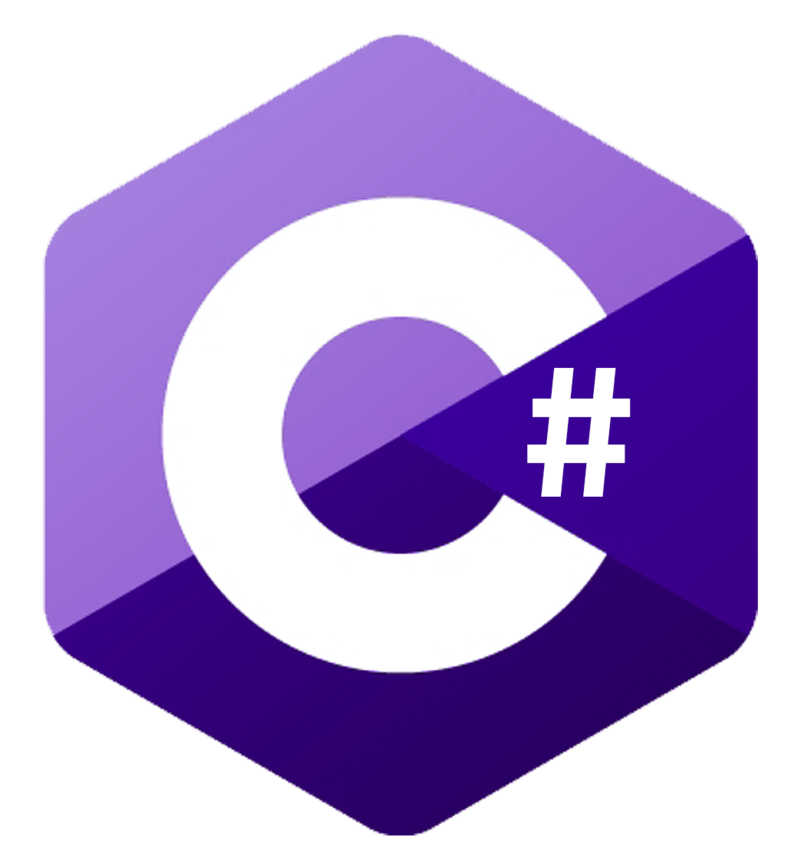
\includegraphics[scale=0.2]{csharp.png}
	\end{center}
	
	\par C\# este un limbaj de programare orientat-obiect conceput de Microsoft la sfârșitul anilor 90. A fost conceput ca un concurent pentru limbajul Java. Ca și acesta, C\# este un derivat al limbajului de programare C++.
	
	\par Eu am folosit acest limbaj de programare pentru scriptare în motorul de joc Unity. Aveam si alte alegeri, cum ar fi Unity Script. Totuși din motivul că deja aveam experiență in C\# și că Unity Script era mult mai puțin folosit în scriptare, am decis să merg cu C\#. În plus, majoritatea documentației e dedicată pentru C\#
	
	\begin{center}
		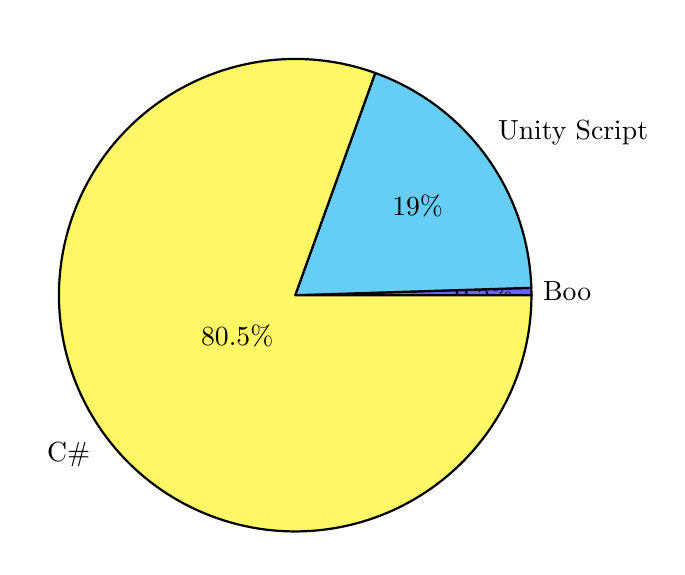
\begin{tikzpicture}
			\pie{0.5/Boo, 19/Unity Script, 80.5/C\#}
		\end{tikzpicture}
	\end{center}
	
	\par În timpul dezvoltării .NET Framework, clasele bibliotecilor au fost scrise într-un cod compilator de sistem dirijat numit "Simple Managed C"(SMC). În ianuarie 1999, Andres Hejlsberg a format o echipă pentru a contrui un limbaj nou numit pe atunci Cool. Microsoft avea de gând să păstreze numele de "Cool" ca nume final pentru acest limbaj, dar a decis să nu o facă din motive de marcă a fabricii. Până a fost anunțat proiectul .NET în îulie 2000 la Professional Developers Conference, limbajul a fost deja redenumit C\#, iar bibliotecile si ASP.NET runtime au fost portate pe C\#.
	
	\par Hejlsberg e un dezvoltator principal pentru C\# și arhitect la Microsoft, fiind parte din echipa de dezvoltare a lui Turbo Pascal, Embarcadero Delphi și Visual J++. În interviuri el a zis ca problemele celor mai mari limbaje de programare a dus la crearea de Common Language Runtime, care dupa, a ajutat cu formarea limbajului C\#.
	
	\par James Gosling, care a creat limbajul de programare Java în 1994, și Bill Joy, un co-fondator al Sun Microsystems, părintele lui Java, au numit C\# o "imitație" de al lui Java. Au fost diferite reacții pentru cele două programe, unii fiind de părere că ambele limbaje au fost o contribuție inutilă pentru programatori și că nu aduceau nimic nou. Hejlsberg a menționat totuși că nu C\# nu e deloc o clonă de a lui Java, ea având ca bază C++.
	
	\par De când a fost lansat C\# 2.0 în noiembrie 2005, limbajele C\# și Java au evoluat pe traiectorii diferite, devenind două limbaje foarte distincte. Una din marile differențe a fost cu implementarea de generice in cele două limbaje. În plus C\# a mai adăugat si extensii LINQ cu lansarea lui C\# 3.0 și suportă "framework"-ul de expresii lambda, extensii de metode și tipuri anonime. Aceste caracteristici au ajutat implementarea programelor în C\# de către programatori.
	
	\resizebox{\textwidth}{!}{%
		\begin{tabular}{
				>{\columncolor[HTML]{EFEFEF}}c |lll}
			\textbf{Versiune}                                                                      & \multicolumn{1}{c}{\cellcolor[HTML]{EFEFEF}\textbf{Data apariție}} & \multicolumn{1}{c}{\cellcolor[HTML]{EFEFEF}\textbf{.NET Framework}}                                                          & \multicolumn{1}{c}{\cellcolor[HTML]{EFEFEF}\textbf{Visual Studio}}              \\ \hline
			\textbf{Versiunea C\# 1.0}                                                             & Ianuarie 2002                                                      & .NET Framework 1.0                                                                                                           & Visual Studio .NET 2002                                                         \\
			\textbf{\begin{tabular}[c]{@{}c@{}}Versiunea C\# 1.1\\ Versiunea C\# 1.2\end{tabular}} & Aprilie 2003                                                       & .NET Framework 1.1                                                                                                           & Visual Studio .NET 2003                                                         \\
			\textbf{Versiunea C\# 2.0}                                                             & Noiembrie 2005                                                     & \begin{tabular}[c]{@{}l@{}}.NET Framework 2.0\\ .NET Framework 3.0\end{tabular}                                              & \begin{tabular}[c]{@{}l@{}}Visual Studio 2005\\ Visual Studio 2008\end{tabular} \\
			\textbf{Versiunea C\# 3.0}                                                             & Noiembrie 2007                                                     & \begin{tabular}[c]{@{}l@{}}.NET Framework 2.0 (Fără LINQ)\\ .NET Framework 3.0 (Fără LINQ)\\ .NET Framework 3.5\end{tabular} & Visual Studio 2008                                                              \\
			\textbf{Versiunea C\# 4.0}                                                             & Aprilie 2010                                                       & .NET Framework 4                                                                                                             & Visual Studio 2010                                                              \\
			\textbf{Versiunea C\# 5.0}                                                             & August 2012                                                        & .NET Framework 4.5                                                                                                           & \begin{tabular}[c]{@{}l@{}}Visual Studio 2012\\ Visual Studio 2013\end{tabular} \\
			\textbf{Versiunea C\# 6.0}                                                             & Iulie 2015                                                         & \begin{tabular}[c]{@{}l@{}}.NET Framework 4.6\\ .NET Core 1.0\\ .NET Core 1.1\end{tabular}                                   & Visual Studio 2015                                                              \\
			\textbf{Versiunea C\# 7.0}                                                             & Martie 2017                                                        & .NET Framework 4.7                                                                                                           & \begin{tabular}[c]{@{}l@{}}Visual Studio 2017\\ version 15.0\end{tabular}       \\
			\multicolumn{1}{l|}{\cellcolor[HTML]{EFEFEF}\textbf{Versiunea C\# 7.1}}                & August 2017                                                        & .NET Core 2.0                                                                                                                & \begin{tabular}[c]{@{}l@{}}Visual Studio 2017\\ version 15.3\end{tabular}       \\
			\multicolumn{1}{l|}{\cellcolor[HTML]{EFEFEF}\textbf{Versiunea C\# 7.2}}                & Noiembrie 2017                                                     &                                                                                                                              & \begin{tabular}[c]{@{}l@{}}Visual Studio 2017\\ version 15.5\end{tabular}       \\
			\multicolumn{1}{l|}{\cellcolor[HTML]{EFEFEF}\textbf{Versiunea C\# 7.3}}                & May 2018                                                           & \begin{tabular}[c]{@{}l@{}}.NET Core 2.1\\ .NET Core 2.2\\ .NET Framework 4.8\end{tabular}                                   & \begin{tabular}[c]{@{}l@{}}Visual Studio 2017 \\ version 15.7\end{tabular}      \\
			\textbf{Versiunea C\# 8}                                                               & Septembrie 2019                                                    & .NET Core 3.0                                                                                                                & \begin{tabular}[c]{@{}l@{}}Visual Studio 2019 \\ version 16.3\end{tabular}     
		\end{tabular}%
	}
	
	
	\subsection{MegaPi}
	
	\begin{center}
		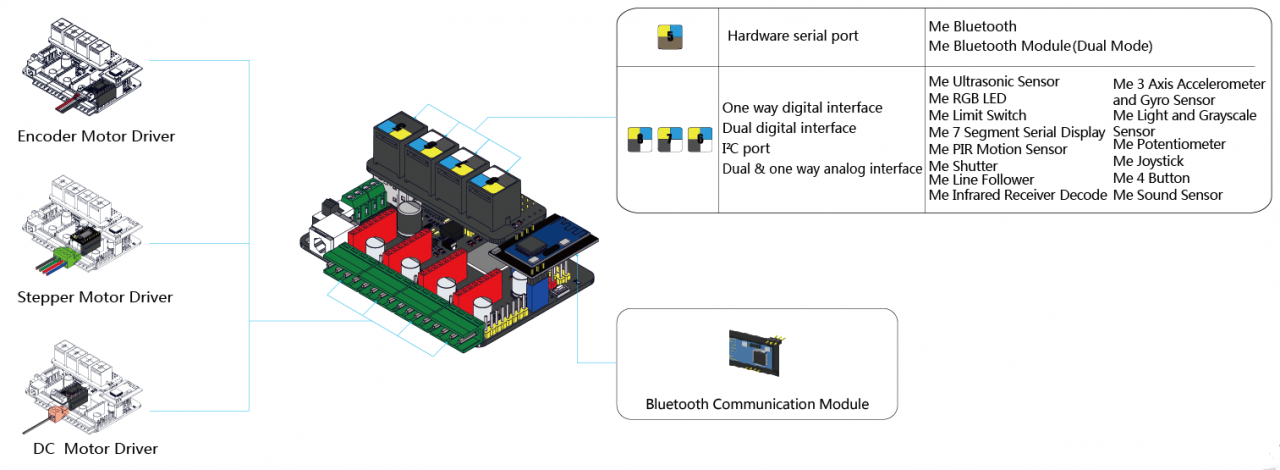
\includegraphics[scale=0.3]{megapi.png}
	\end{center}
	
	\par MegaPi e o placă de control principală destinată în special pentru creatori și de a fi folosit în educație sau alte de genul. Este bazat pe Arduino MEGA 2560 și suportă programarea cu Arduino IDE fără nici o problemă.
	
	\par Aveam de ales între Arduion, Raspberry Pi si acest MegaPi pentru controlarea robotului. Din cauză că robotul găsit a venit cu un MegaPi inclus cu el e singurul motiv pentru care l-am păstrat pe robotul curent ales. A fost si ușor de invațat de folosit deoarece am putut investiga "firmware"-ul original și robotul era conceput de la început să lucreze cu acest MegaPi. 
	
	\par MegaPi poate fi impărtit in 6 zone de funcțiune, ceea ce iți permite să te conectezi cu diferite module, motoare și senzori și pentru a realiza conecțiune "wireless". MegaPi e capabil de a avea 10 servo motoare sau 8 DC motoare în mod simultan. E ideal pentru diverse proiecte cu roboți.
	
	\begin{itemize}
		\item Microcontroller: ATMEGA2560-16AU
		\item Input Voltage: DC 6V-12V
		\item Operating Voltage: DC 5V
		\item I/O Pins: 43
		\item Serial Ports: 3
		\item I2C Interface: 1
		\item SPI Interface: 1
		\item Analog Input Pins: 15
		\item DC Current per I/O Pin: 20mA
		\item Flash Memory: 256KB
		\item SRAM: 8KB
		\item EEPROM: 4KB
		\item Clock Speed: 16 MHz
		\item Dimension: 85*63mm
	\end{itemize}
	
	\subsection{Bluetooth}
	
	\begin{center}
		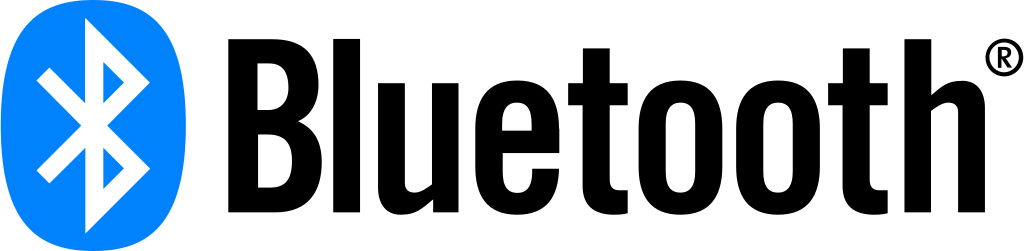
\includegraphics[scale=0.25]{bluetoothlogo.png}
	\end{center}
	
	\par Bluetooth este un set de specificații (un standard) pentru o rețea personală (engleză: personal area network, PAN) fără fir (wireless), bazată pe unde radio. Bluetooth mai este cunoscut ca și standardul IEEE 802.15.1. Prin tehnologia Bluetooth se elimină firele și cablurile între dispozitive atât staționare cât și mobile, facilitează atât comunicațiile de date cât și pe cele vocale și oferă posibilitatea implementării unor rețele ad-hoc și a sincronizării între diverse dispozitive.
	
	\par Modulul de Bluetooth din robot e folosit în special pentru transmitere de date wireless la distanțe mici. Se poate connecta ușor la alte dispozitive cu Bluetooth, ceea ce include telefoane si calculatoare. În plus, modulul permite transmisia de date între 2 module ca să nu se complice cu fire și in caz că e nevoie de spațiu. Folosind modulul de Bluetooth se poate controla roboți MakeBlock (robotul nostru fiind parte din această categorie) cu telefonul sau calculatorul (Bluetooth Version 4.0).
	
	\begin{center}
		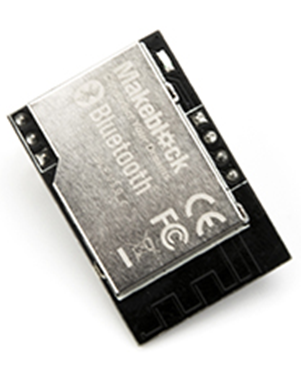
\includegraphics[scale=0.25]{bluetoothmodule.png}
	\end{center}

	\par Specificația Bluetooth a fost formulată pentru prima dată în 1994 de Sven Mattisson și Jaap Haartsen, muncitori în orașul Lund, Suedia, la divizia de telefonie mobilă a companiei Ericsson. La 20 mai 1998 a fost fondată gruparea Bluetooth Special Interest Group (SIG), care are rolul de a gestiona tehnologia Bluetooth și de a urmări evoluția acestei tehnologii.
	
	\begin{itemize}
		\item 1994: crearea standardului de către de Sven Mattisson și Jaap Haartsen la compania Ericsson
		\item 1998: IBM, Intel, Nokia și Toshiba sunt partenere cu Ericsson pentru formarea grupului Bluetooth Special Interest Group (SIG)
		\item 1999: apare specificația 1.0, apoi 1.0B
		\item 1999: Ericsson a lansat primul telefon dotat cu Bluetooth, modelul Ericsson T39
		\item 2006: cea de-a doua generație Bluetooth v2.0 (apoi V2.1 în 2007). Noul standard a inclus și tehnologia ultrawideband UWB
		\item 2009: standardul Bluetooth 3.0 și varianta HS (High Speed)
		\item 2010: apariția Bluetooth 4.0 mai puternică și mai puțin consumatoare de energie, Bluetooth Low Energy, (BLE) sau Wibree
		\item 2013: lansarea versiunii 4.1
		\item 2016: lansarea versiunii 5
	\end{itemize}
	
	\par Printr-o rețea Bluetooth se poate face schimb de informații între diverse aparate precum telefoane mobile, laptop-uri, calculatoare personale, imprimante, camere foto și video digitale sau console video prin unde radio criptate (sigure) și de rază mică, desigur numai dacă aparatele respective sunt înzestrate și cu Bluetooth.
	
	\par Aparatele care dispun de Bluetooth comunică între ele atunci când se află în aceeași rază de acțiune. Ele folosesc un sistem de comunicații radio, așa că nu este nevoie să fie poziționate față în față pentru a transmite; dacă transmisia este suficient de puternică, ele pot fi chiar și în camere diferite.
	
	\subsection{Ultimate 2.0 – 10 in 1 Robot Kit}
	
	\begin{center}
		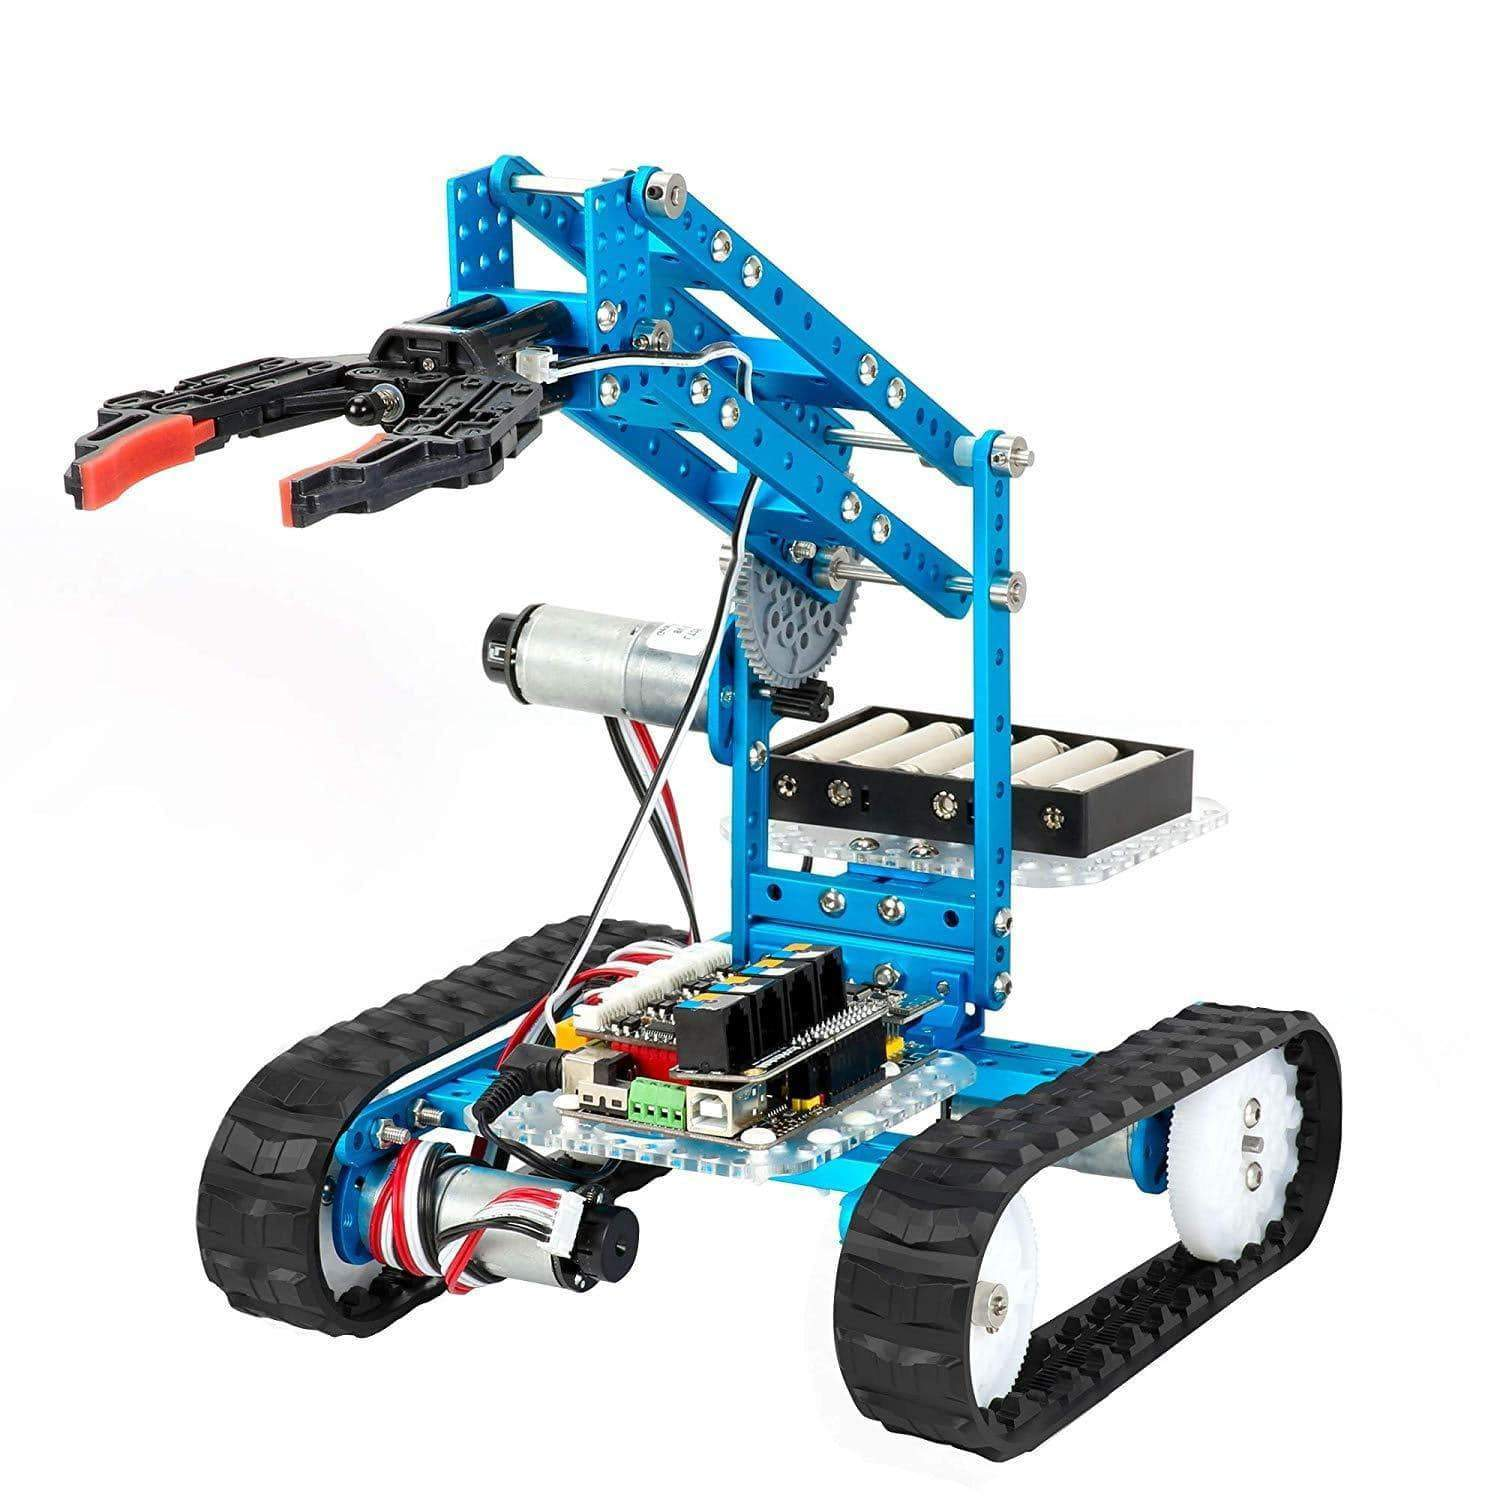
\includegraphics[scale=0.15]{robot.jpg}
	\end{center}
	
	\par Ultimate 2.0 este un kit de robot avansat și programabil care cuprinde mai mult de 550 de părți mecanice și module electronice pentru 10 roboți diferiți personalizați, cât și pentru alte idei proprii. Compatibil cu platforma "maker" și Arduino, kit-ul te lasă să iți folosești imaginația. E ideal pentru un robot entuzias și pentru construit proiecte interesante prin a aduce ideile la realitate.
	
	\section{Exemple de funcționalitate și cod}
	
	\par Avem o diagramă a întregului proiect care explică conecțiunile dintre toate componentele folosite cât și o bază a claselor folosite prin proiect. 
	
	\begin{center}
		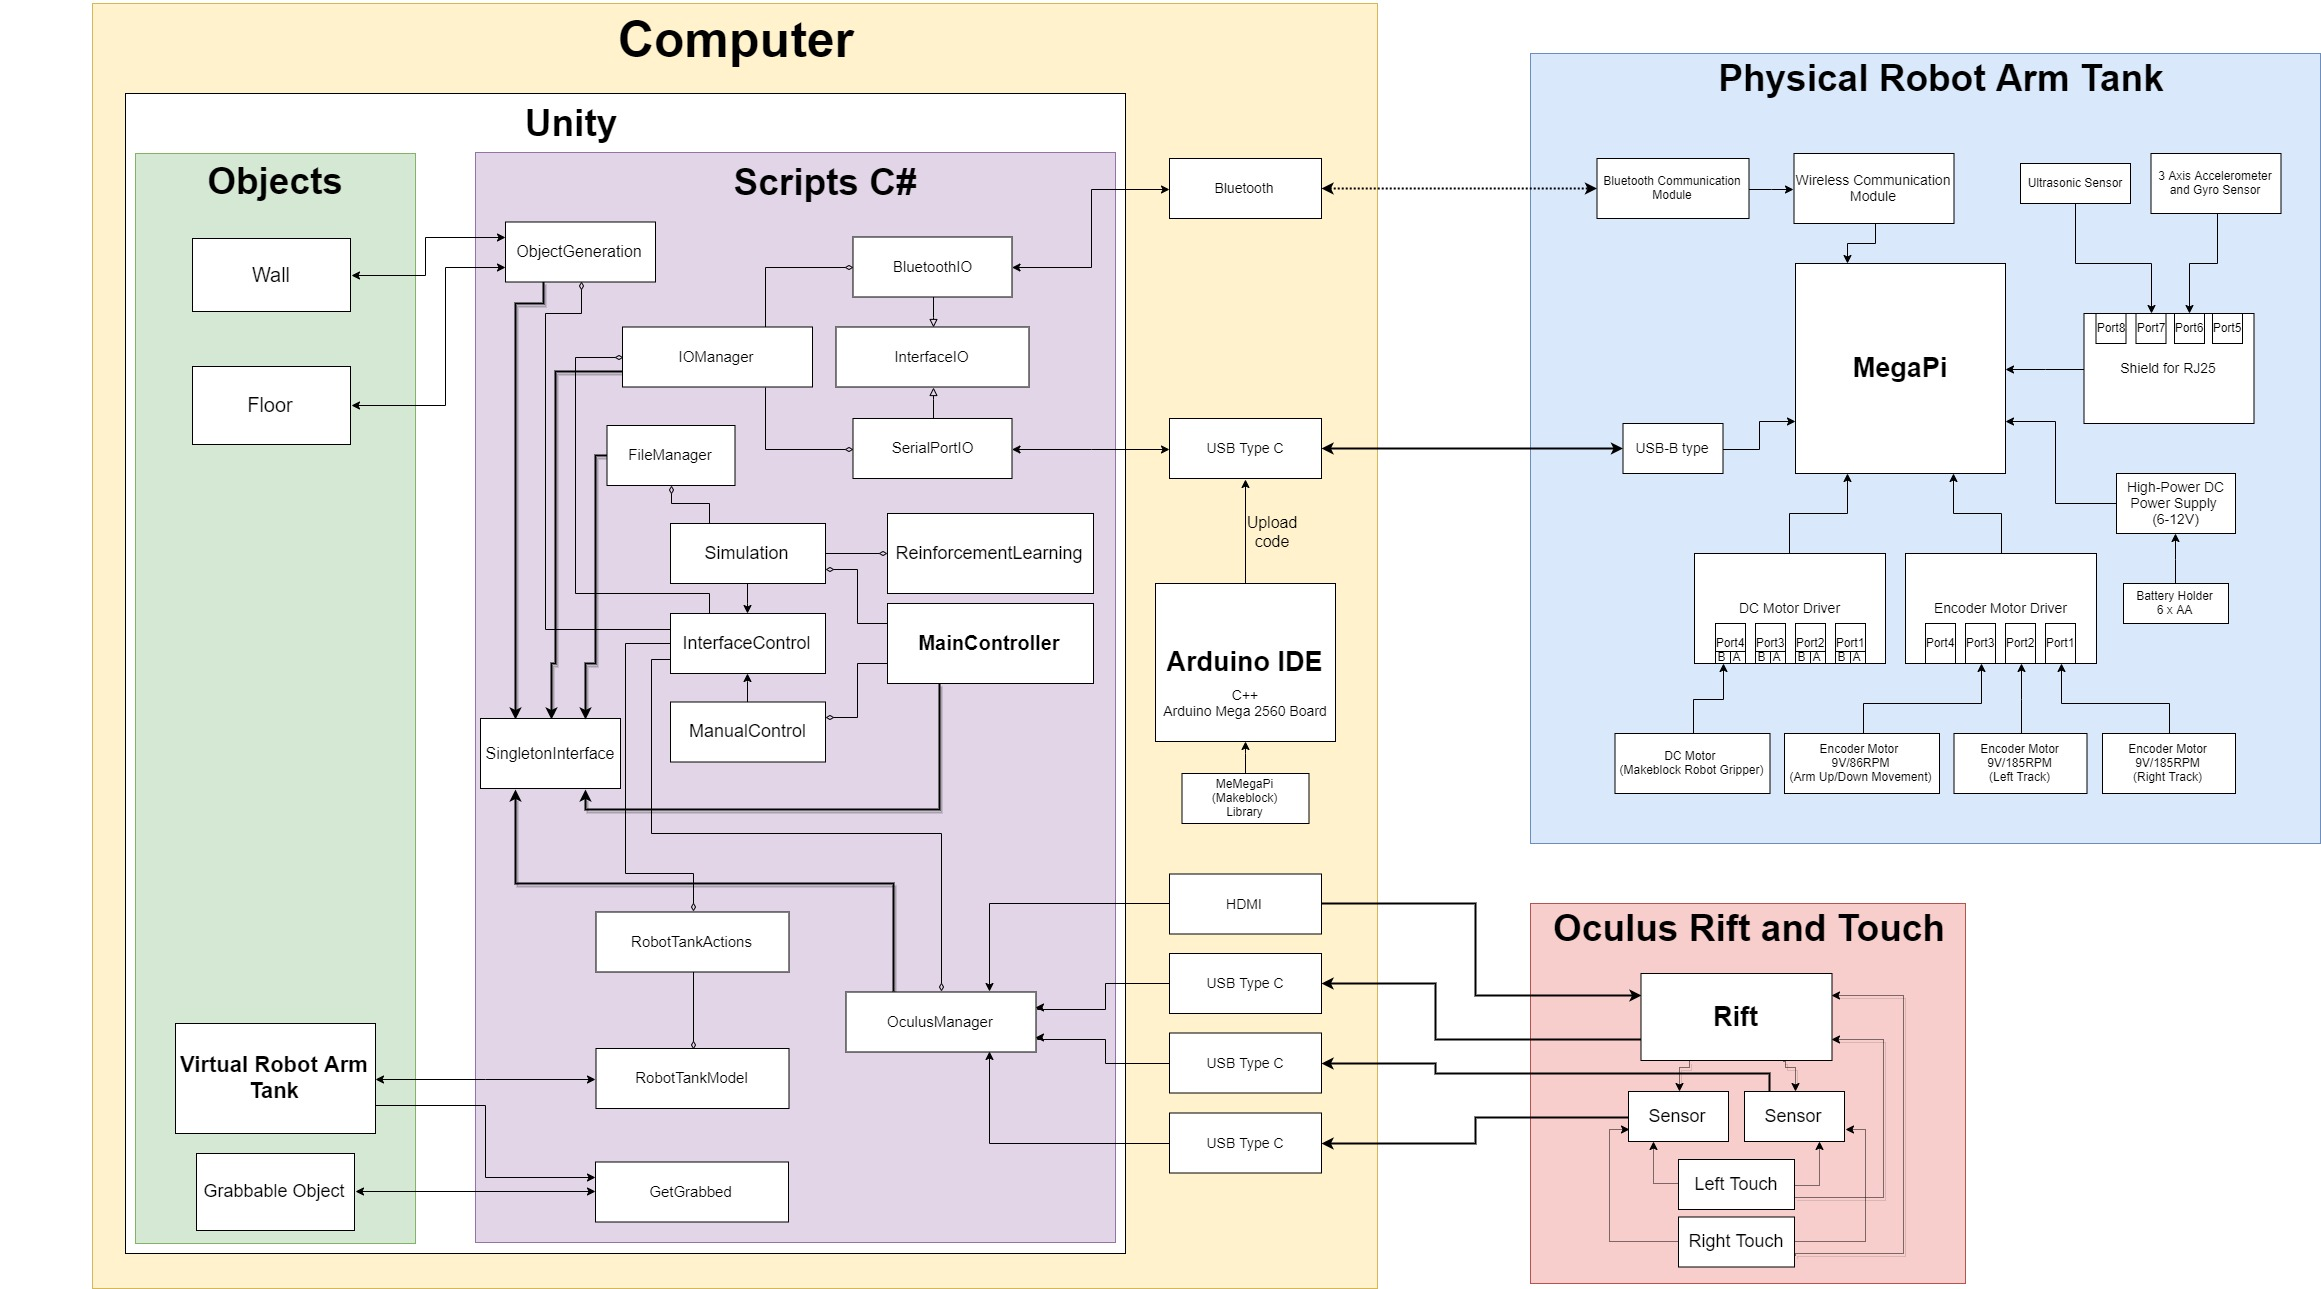
\includegraphics[scale=0.15]{diagram.jpg}
	\end{center}
	
	\par Tot codul afișat mai jos se ocupă complet de a contola mișcările robotului în funcție de ce date i se transmite. El așteaptă să primească date, iar atunci când primeste el va verifica byte cu byte unde trebuie să se ducă prin cod și ce trebuie să facă. Dacă primul byte din cod nu este una dintre acțiuni, atunci nu se v-a executa nimic, altfel încearcă să execute acțiunea dată până la capăt.
	
	\begin{lstlisting}[language=C++, caption=Firmware pentru robot]
	#include <MeMegaPi.h>
	
	MeMegaPiDCMotor dc;
	MeEncoderOnBoard Encoder_1(SLOT1);
	MeEncoderOnBoard Encoder_2(SLOT2);
	MeEncoderOnBoard Encoder_3(SLOT3);
	
	int data;
	
	void setup() 
	{
	Serial.begin(9600);
	dc.reset(PORT4B);
	}
	
	int getSignByCharacter(int character)
	{
	if(character == 'N')
	{
	return -1;
	}
	return 1;
	}
	
	int awaitRead()
	{
	while(Serial.available() == 0) { }
	return Serial.read(); 
	}
	
	int constrainToMaxAndMinSpeed(int speed)
	{
	const int maximumSpeed = 255;
	const int minimumSpeed = 100;
	
	if (speed > maximumSpeed)
	{
	return maximumSpeed;
	}
	
	if (speed < minimumSpeed)
	{
	return minimumSpeed;
	}
	return speed;
	}
	
	int getMotorSpeed()
	{
	int motorSpeedSign = awaitRead(); // sign
	int motorSpeed = awaitRead(); // part 1
	int motorSpeedPart2 = awaitRead(); // part 2
	motorSpeed = constrainToMaxAndMinSpeed(motorSpeed + motorSpeedPart2);
	return motorSpeed * getSignByCharacter(motorSpeedSign);
	}
	
	void notMoveAction() 
	{
	Encoder_1.setMotorPwm(0);
	Encoder_2.setMotorPwm(0);
	}
	
	void notArmAction() 
	{
	Encoder_3.setMotorPwm(0);
	}
	
	void notClawAction() 
	{
	dc.run(0);
	}
	
	void moveAction()
	{
	Encoder_1.setMotorPwm(getMotorSpeed());// R
	Encoder_2.setMotorPwm(getMotorSpeed());// L
	}
	
	void clawAction()
	{
	dc.run(getMotorSpeed());
	}
	
	void armAction()
	{
	Encoder_3.setMotorPwm(getMotorSpeed());// Arm
	}
	
	// m - don't use movement; M - move; A - arm(up/down movement); a - don't use arm; C - claw; c - don't use claw; N - Negative
	void loop() 
	{
	data = awaitRead();
	if(data == 'M')
	{
	moveAction();
	} 
	else if (data == 'm')
	{
	notMoveAction();
	} 
	else if (data == 'C')
	{
	clawAction();
	} 
	else if (data == 'c')
	{
	notClawAction();
	} 
	else if (data == 'A')
	{
	armAction();
	}
	else if (data == 'a')
	{
	notArmAction();
	}
	}
	\end{lstlisting}
	
	\par Din partea programului de pe calculator, acesta ia datele din VR și, după ce le procesează, le transmite la robot print-o listă de bytes. Aici avem un exemplu de cum se transmite o comandă pentru mișcatul de șine.
	
	\begin{lstlisting}[language=C++, caption=Transmiterea datelor]
	float forwardSpeedValue = yNomalized * fastestMovementSpeed;
	float rotationSpeedValue = xNomalized * fastestMovementSpeed;
	
	if (forwardSpeedValue != 0 && rotationSpeedValue != 0)
	{
	float motor1Speed = ((forwardSpeedValue - rotationSpeedValue) / 2) * speedMultiplyer; // R part 1
	float motor1SpeedPart2 = motor1Speed; // R part 2
	
	float motor2Speed = (-(forwardSpeedValue + rotationSpeedValue) / 2) * speedMultiplyer; // L part 1
	float motor2SpeedPart2 = motor2Speed; // L part 2
	
	char motor1SpeedSign = 'P'; // R sign
	char motor2SpeedSign = 'P'; // L sign
	
	if (motor1Speed < 0)
	{
	motor1Speed *= -1;
	motor1SpeedPart2 *= -1;
	motor1SpeedSign = 'N';
	}
	
	if (motor2Speed < 0)
	{
	motor2Speed *= -1;
	motor2SpeedPart2 *= -1;
	motor2SpeedSign = 'N';
	}
	
	char motor1SpeedSend = ((char)((int)(motor1Speed))); // R part 1
	char motor1SpeedPart2Send = ((char)((int)(motor1SpeedPart2))); // R part 2
	
	char motor2SpeedSend = ((char)((int)(motor2Speed))); // L part 1
	char motor2SpeedPart2Send = ((char)((int)(motor2SpeedPart2))); // L part 2
	
	string completeSend = "M" + motor1SpeedSign + motor1SpeedSend + motor1SpeedPart2Send +
	motor2SpeedSign + motor2SpeedSend + motor2SpeedPart2Send;
	Debug.Log(completeSend);
	serial.Write(completeSend);
	}
	else
	{
	serial.Write("m");
	}
	\end{lstlisting}
	
	\par În același timp, noi folosim datele din VR și pentru a mișca robotul din lumea virtuală.
	
	\begin{lstlisting}[language=C++, caption=Mișcarea robotului virtual]
	void MoveLeftRight()
	{
	var wholeBodyAngles = rotationBody.transform.localRotation.eulerAngles;
	float rotateToValue = wholeBodyAngles.z - rotationSpeed * leftThumbstickLeftRight;
	rotationBody.transform.localRotation = Quaternion.Euler(wholeBodyAngles.x, wholeBodyAngles.y, rotateToValue);
	}
	
	void MoveForwardBackwards()
	{
	var wholeBodyPosition = movementBody.transform.localPosition;
	float moveToValue = wholeBodyPosition.y + movementSpeed * leftThumbstickUpDown;
	movementBody.transform.localPosition = new Vector3(wholeBodyPosition.x, moveToValue, wholeBodyPosition.z);
	this.transform.position = movementBody.transform.position;
	movementBody.transform.localPosition = new Vector3(0, 0, 0);
	}
	\end{lstlisting}
	
	\pagebreak
	\section{Bibliografie}
	
	\begin{itemize}
		\item \url{https://en.wikipedia.org/wiki/Unity_(game_engine)}
		\item \url{https://en.wikipedia.org/wiki/C_Sharp_(programming_language)}
		\item \url{http://learn.makeblock.com/en/megapi/}
		\item \url{http://learn.makeblock.com/en/bluetooth-modulesingle-mode/}
		\item \url{https://ro.wikipedia.org/wiki/Bluetooth}
		\item \url{https://www.makeblock.com/steam-kits/mbot-ultimate}
	\end{itemize}
	
\end{document}